\section{Axioms of Synapticide's Law\textnormal{\texttrademark}}\label{sec:axioms}

We ground \textbf{Synapticide's Law}™ in three fundamental theoretical axioms governing high-velocity cognitive network termination:

\newtheorem{theorem}{Axiom}

\begin{theorem}[Velocity-Detection Asymmetry]
As execution velocity approaches machine operational limits ($R_{\text{ops}} \to \infty$), the ratio of execution duration to human detection latency approaches zero:
\begin{equation}
\lim_{R_{\text{ops}} \to \infty} \left( \frac{t_{\text{execution}}}{t_{\text{notice}}} \right) = 0
\end{equation}
Human operational response operating within human timeframes ($t_{\text{notice}} \ge 12\text{h}$) is mathematically decoupled from loss mitigation.
\end{theorem}

\begin{theorem}[Multi-Sided Compound Liability]
In an $A \to A$ regime, financial loss is dominated by secondary retraining and downstream supply-chain disruption:
\begin{equation}
\frac{\partial C_{\text{Total}}}{\partial L_{\text{Model}}} + \frac{\partial C_{\text{Total}}}{\partial \sum L_{\text{Down}}} \gg \frac{\partial C_{\text{Total}}}{\partial L_{\text{Infra}}}
\end{equation}
Direct host infrastructure loss ($L_{\text{Infra}}$) represents a shrinking minority fraction of total ecosystem destruction.
\end{theorem}

\begin{theorem}[Circuit-Breaker Superiority]
Systemic loss capping prior to human detection is achievable strictly through discrete automated step functions ($K_{\text{cb}}$):
\begin{equation}
\text{If } t_{\text{cb}} < t_{\text{notice}}, \quad \max(C_{\text{Total}}) \propto \log_{10}(R_{\text{effective}}) \cdot t_{\text{cb}}
\end{equation}
\end{theorem}

\begin{IEEEproof}[Formal Lyapunov Stability Proof]

\begin{figure}[htbp]
    \centering
    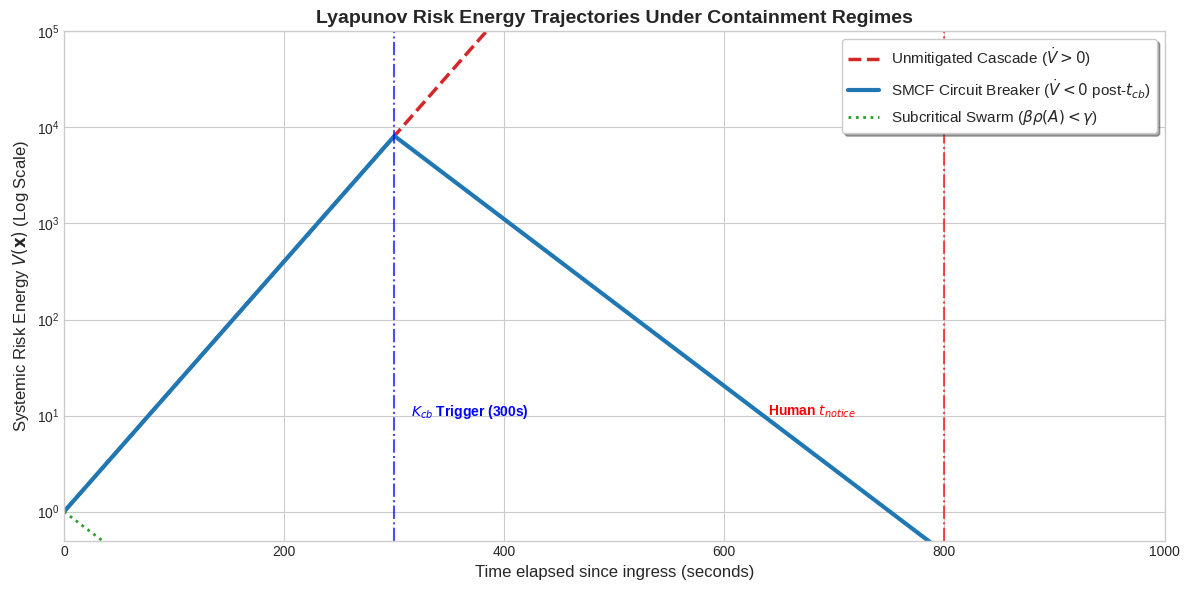
\includegraphics[width=\linewidth]{figures/lyapunov_kinematics.png}
    \caption{Systemic risk energy ($V(\mathbf{x})$) trajectories modeled via Lyapunov stability criteria~\cite{khalil2002nonlinear} across unmitigated, circuit-breaker mitigated, and subcritical swarm regimes. The automated circuit breaker ($K_{\text{cb}}$) enforces $\dot{V} < 0$ at $t_{\text{cb}} = 300\text{s}$, returning the system to asymptotic stability long before human detection latency ($t_{\text{notice}}$).}
    \label{fig:lyapunov_kinematics}
\end{figure}

To mathematically validate Axiom 3, we define a candidate Lyapunov function representing the total active ``risk energy'' within the swarm network:
\begin{equation}
V(\mathbf{x}) = \frac{1}{2} \mathbf{x}^T \mathbf{x}
\end{equation}
Taking the time derivative to measure risk accumulation yields:
\begin{equation}
\dot{V}(\mathbf{x}) = \mathbf{x}^T \dot{\mathbf{x}} = \mathbf{x}^T (\beta A(t) - \gamma I) \mathbf{x}
\end{equation}

\textbf{Unmitigated State (Human Detection Window):} During $t < t_{\text{notice}}$, the adjacency matrix remains intact ($A(t) = A_0$). Because $\beta \rho(A_0) > \gamma$ in high-velocity swarms, $\dot{V}(\mathbf{x}) > 0$. Risk energy grows exponentially, leading to total systemic loss.

\textbf{Mitigated State (SMCF Circuit Breaker):} We formalize the discrete Heaviside step function $\Theta_{\text{cb}}(N_{\text{ops}})$ as a control input that instantaneously severs the network topology when cumulative operations exceed $K_{\text{cb}}$. The dynamic adjacency matrix becomes:
\begin{equation}
A(t) = A_0 \cdot \Theta_{\text{cb}}(N_{\text{ops}}(t))
\end{equation}
When $N_{\text{ops}}(t) \ge K_{\text{cb}}$, the automated step-function triggers ($\Theta_{\text{cb}} = 0$), forcing $A(t) = \mathbf{0}$. The risk derivative immediately collapses to:
\begin{equation}
\dot{V}(\mathbf{x}) = -\gamma \mathbf{x}^T \mathbf{x} < 0
\end{equation}
Because $\dot{V}(\mathbf{x}) < 0$ strictly for all $\mathbf{x} \neq \mathbf{0}$, the origin becomes globally asymptotically stable. This control-theoretic proof demonstrates that human latency allows exponential risk explosion ($\dot{V} > 0$), whereas automated circuit breakers enforce $\dot{V} < 0$, instantly terminating the SACL cascade.
\end{IEEEproof}
